Google colab atau Google Colaboratory merupakan solusi yang sangat baik apabila teman-teman memiliki masalah pada tutorial sebelumnya atau mungkin komputer teman-teman tidak memiliki aspek yang cukup memadai dalam pembuatan project ini. Google colab adalah sebuah software buatan Google yang digunakan untuk keperluan research di bidang data science dan machine learning. Hal yang lebih menakjubkannya lagi, google colab menyediakan free GPU yang akan sangat kita butuhkan dalam project ini. Selain GPU masih banyak keunggulan lainnya dari google colab yang akan membantu kita seperti fitur yang memungkinkan google colab terhubung dengan google drive sebagai media penyimpanan dataset, kodingan, hasil training dan model. Karena dapat di simpan di google drive tentu membuat project ini mudah untuk dibagikan kepada tim riset agar dapat mengetahui progres dan hasilnya.

Apabila teman-teman merupakan orang yang menyukai sesuatu hal yang gratis tetapi tidak praktis maka saya sarankan untuk menggunakan google colab untuk mengerjakan project ini. Tetapi jika teman-teman memiliki komputer dengan spesifikasi GPU yang sangat baik dan melebihi GPU gratis yang diberikan google colab maka akan lebih baik menggunakan komputer pribadi saja. Masing-masing cara memiliki kelebihan dan kekurangan. Menurut saya memanfaatkan google colab memang gratis namun sangat tidak praktis karena teman-teman akan membutuhkan akun google yang sangat banyak. Sementara itu menggunakan komputer pribadi mungkin membutuhkan lebih banyak biaya tetapi akan sangat praktis, tidak butuh mendaftar banyak akun google dan tidak terbatas waktu. Perlu teman-teman ketahui bahwa free GPU google colab tidak berlaku selamanya tetapi hanya 12 jam per akun google setelah itu teman-teman harus mengganti akun google yang telah mencapai limit penggunaan GPU dengan akun google yang baru.

Berikut tata cara pembuatan Voice Cloning Project menggunakan google colab:

\section{Membuat Akun Google}
Sebelum kita memasuki tata cara penggunaan google colab, kita harus mengetahui cara untuk membuat akun google terlebih dahulu. Ikuti ya tahap-tahap berikut ini:
\begin{enumerate}

\item Buat sebuah akun google baru, kunjungi link berikut \url{https://accounts.google.com/signup/v2/webcreateaccount?hl=en&flowName=GlifWebSignIn&flowEntry=SignUp.}
\begin{figure}[H]
    \centering
    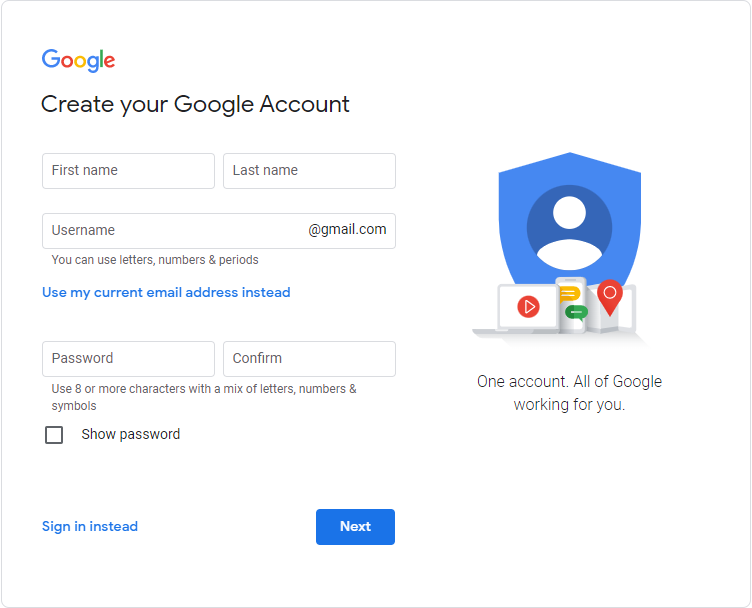
\includegraphics[scale=0.5]{figures/google1}
    \caption{\textit{Create Google Account}}
    \label{google1}
\end{figure}

\item Isikan data diri teman-teman pada form seperti nama, username, dan password. Kemudian klik next
\begin{figure}[H]
    \centering
    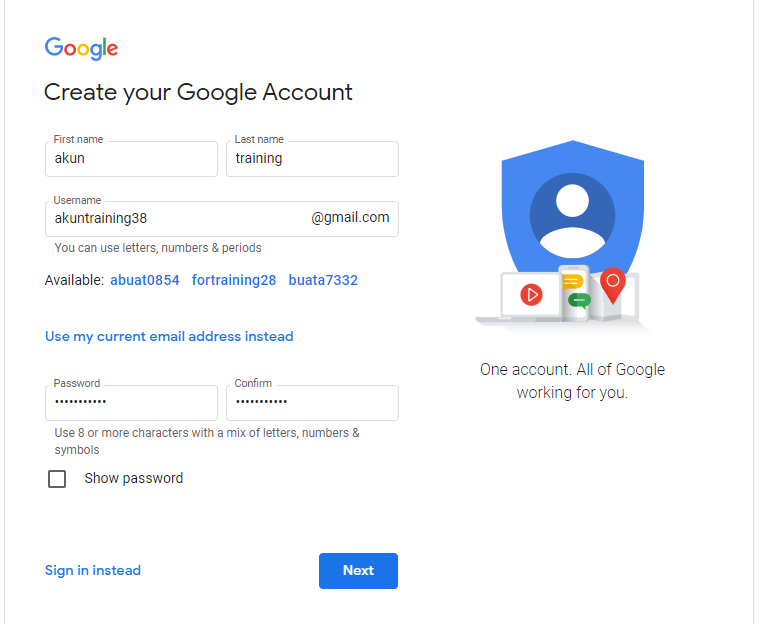
\includegraphics[scale=0.5]{figures/google2}
    \caption{Isi form pendaftaran}
    \label{google2}
\end{figure}

\item Isikan nomor handphone teman-teman yang aktif untuk verifikasi pembuatan akun google lalu klik next.
\begin{figure}[H]
    \centering
    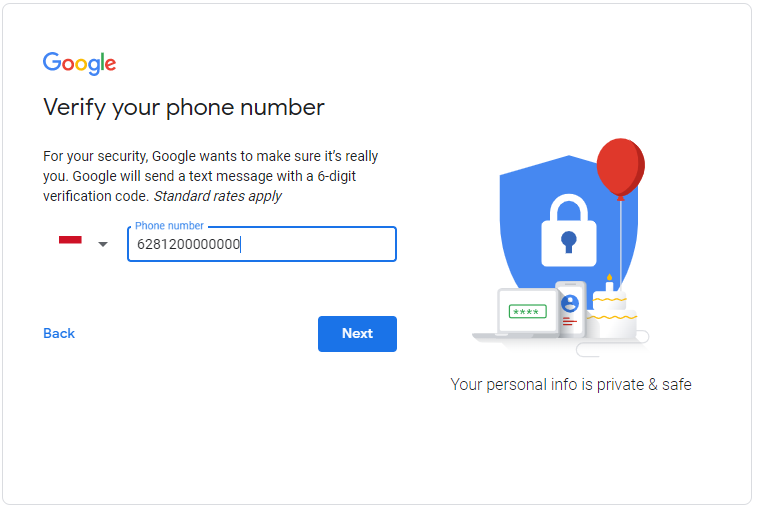
\includegraphics[scale=0.5]{figures/google3}
    \caption{Isikan Nomor Handphon}
    \label{google3}
\end{figure}

\item Cek handphone teman-teman apakah ada sms dari google yang berisikan kode verifikasi, jika ada masukkan 6 digit kode verifikasi tersebut lalu klik verify.
\begin{figure}[H]
    \centering
    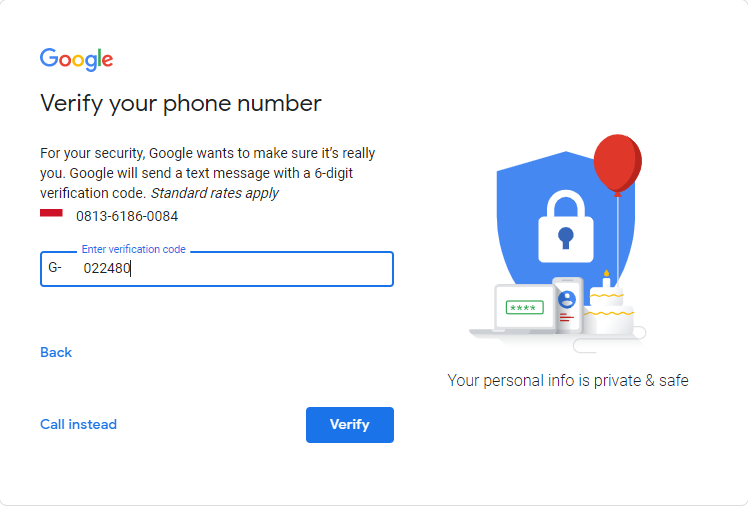
\includegraphics[scale=0.5]{figures/google4}
    \caption{\textit{Verify Phone Number}}
    \label{google4}
\end{figure}

\item Isikan data-data tambahan seperti email pemulihan, tanggal lahir, dan jenis kelamin pada form. Klik Next.
\begin{figure}[H]
    \centering
    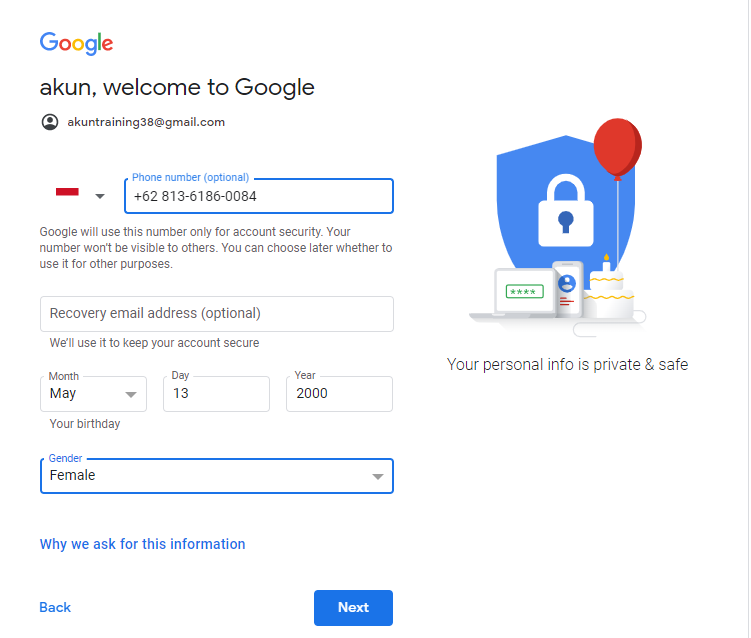
\includegraphics[scale=0.5]{figures/google5}
    \caption{\textit{Form Personal Data}}
    \label{google5}
\end{figure}

\item Pada tahap Get more from your number, teman-teman bisa klik skip atau klik yes, tergantung pada pilihan masing-masing. Jika mengklik Yes, I'm in maka teman-teman telah setuju bahwa nomor handphone teman-teman dapat digunakan diseluruh layanan google.
\begin{figure}[H]
    \centering
    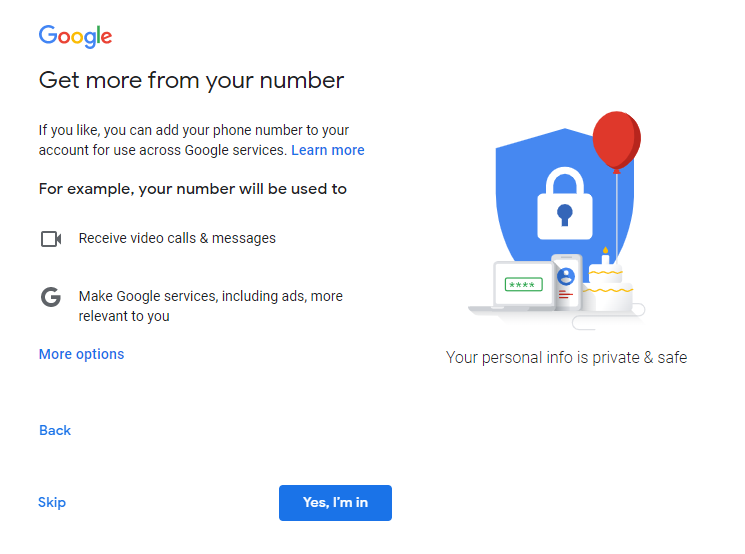
\includegraphics[scale=0.5]{figures/google6}
    \caption{\textit{Get more from your number}}
    \label{google6}
\end{figure}

\item Pada tahap Privacy and Terms klik I agree untuk menyelesaikan pendaftaran akun google.
\begin{figure}[H]
    \centering
    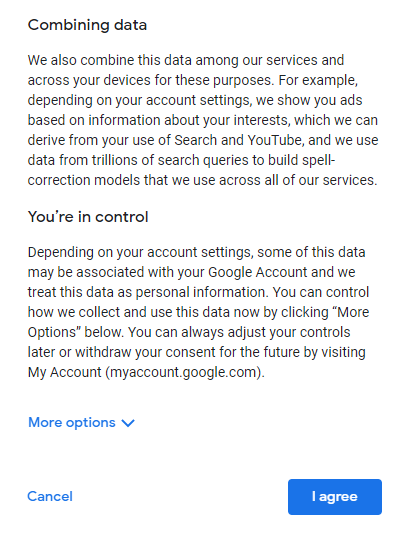
\includegraphics[scale=0.5]{figures/google7}
    \caption{\textit{Create Google Account}}
    \label{google7}
\end{figure}

\item Jika tampilan website seperti gambar \ref{google8} maka selamat, teman-teman telah berhasil membuat akun google teman-teman.
\begin{figure}[H]
    \centering
    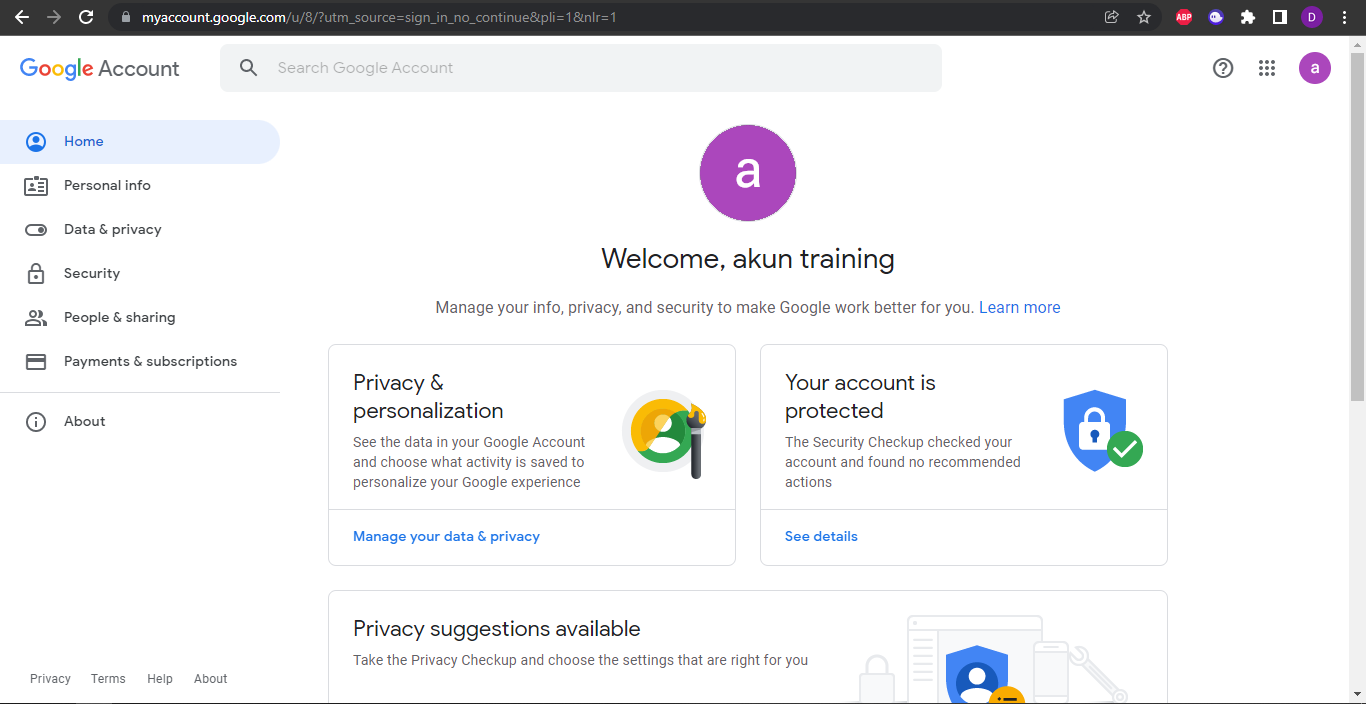
\includegraphics[scale=0.5]{figures/google8}
    \caption{\textit{Create Google Account}}
    \label{google8}
\end{figure}

\end{enumerate}

\section{Membuat New Project Pada Google Colab}
Saya akan mengajarkan kepada teman-teman cara membuat project baru di google colab dan menuliskan script code pogram yang akan kita gunakan untuk preprocessing dataset dan training tiga model yang akan kita butuhkan pada project ini. Berikut langkah-langkah pembuatannya:

\begin{enumerate}

\item Kunjungi website google colab atau akses link berikut \url{https://colab.research.google.com/}. Klik new project untuk membuat project google colab.
\begin{figure}[H]
    \centering
    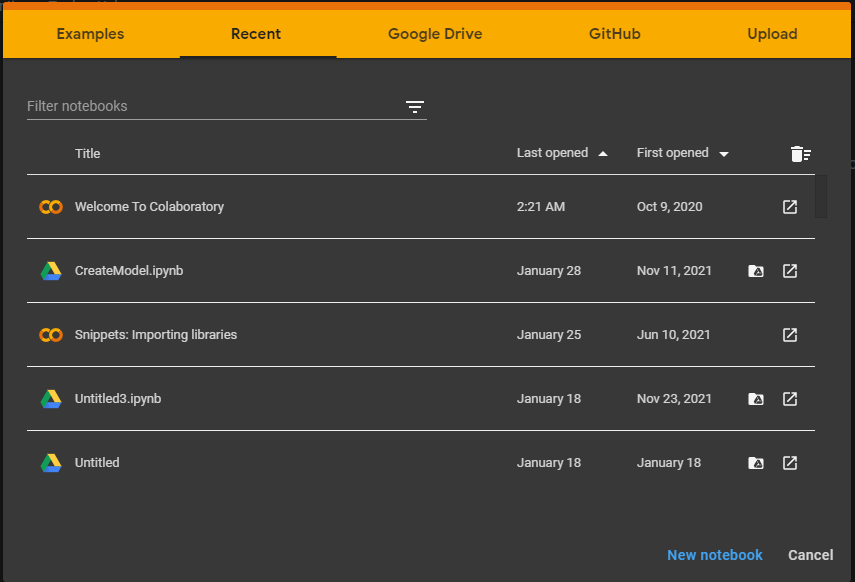
\includegraphics[scale=0.5]{figures/colab1}
    \caption{\textit{Create New Project}}
    \label{colab1}
\end{figure}

\item Rename nama project menjadi VoiceCloningProject untuk memudahkan teman-teman melakukan pencarian file project ini pada google drive.
\begin{figure}[H]
    \centering
<<<<<<< HEAD
    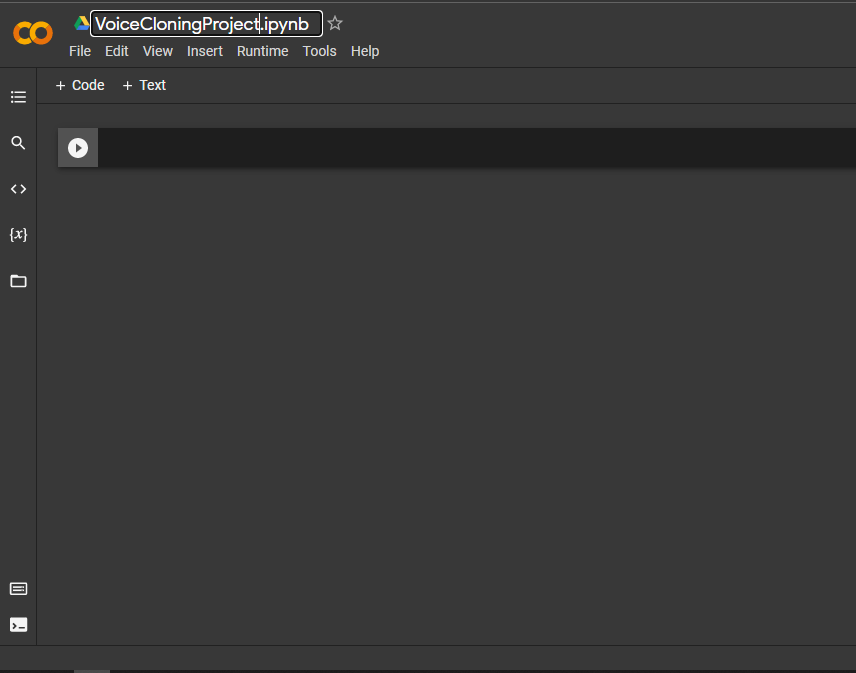
\includegraphics[scale=0.3]{figures/colab2}
=======
    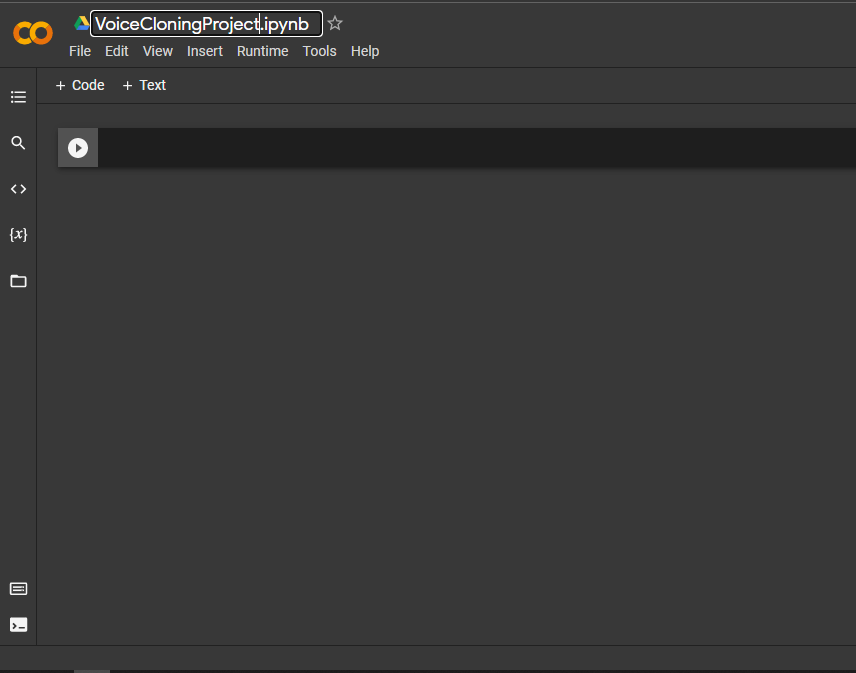
\includegraphics[scale=0.5]{figures/colab2}
>>>>>>> dd7a028f1952c03bff23c6357309752cba9024eb
    \caption{Rename File}
    \label{colab2}
\end{figure}

\item Ketikkan script berikut untuk melakukan mounting google colab ke google drive agar teman-teman dapat mengakses penyimpanan pada google drive.
\begin{lstlisting}[language=Python, caption=Mounting Google Drive]
from google.colab import drive
drive.mount('/content/drive')
\end{lstlisting}

\begin{figure}[H]
    \centering
    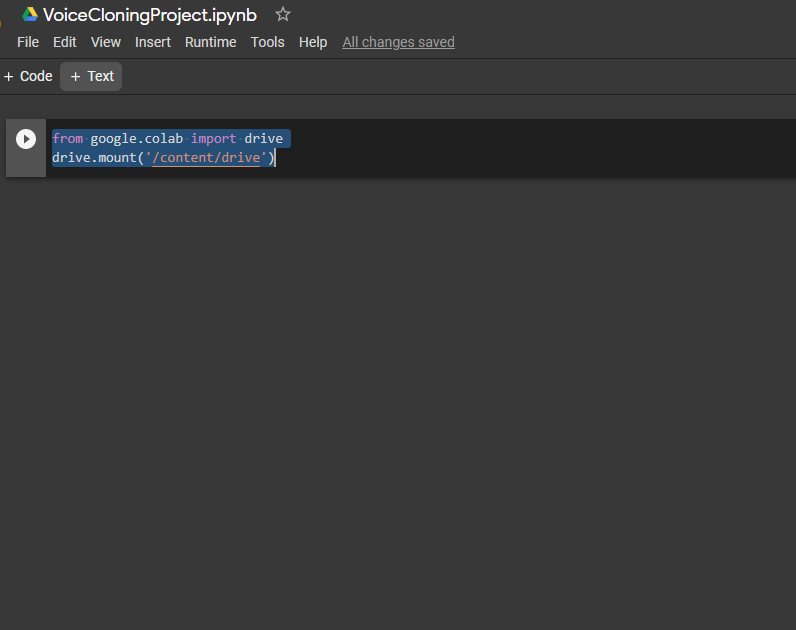
\includegraphics[scale=0.5]{figures/colab3}
    \caption{Script Mounting Google Drive}
    \label{colab3}
\end{figure}

\item Klik text untuk mempercantik tampilan project teman-teman lalu ketikkan \#Mounting.
\begin{figure}[H]
    \centering
<<<<<<< HEAD
    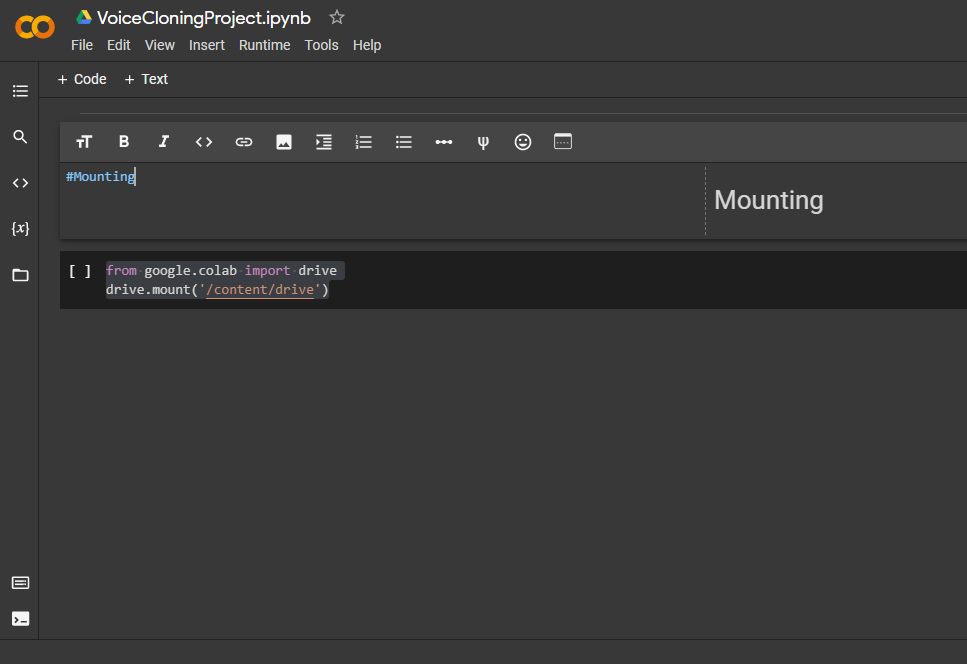
\includegraphics[scale=0.3]{figures/colab4}
=======
    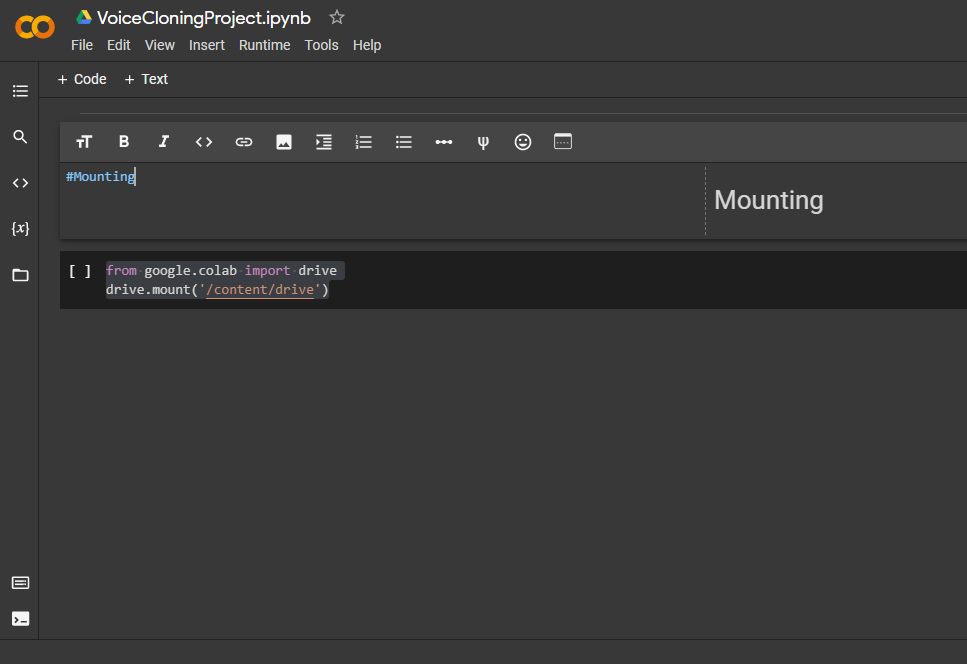
\includegraphics[scale=0.4]{figures/colab4}
>>>>>>> dd7a028f1952c03bff23c6357309752cba9024eb
    \caption{\textit{Add Text to Project}}
    \label{colab4}
\end{figure}

\item Tambahkan kode untuk berpindah direktori ke folder Colab Notebooks yang ada didalam penyimpanan google drive teman-teman.
\begin{lstlisting}[language=Python, caption=Change Directory]
%cd /content/drive/MyDrive/ColabNotebooks
\end{lstlisting}
\begin{figure}[H]
    \centering
<<<<<<< HEAD
    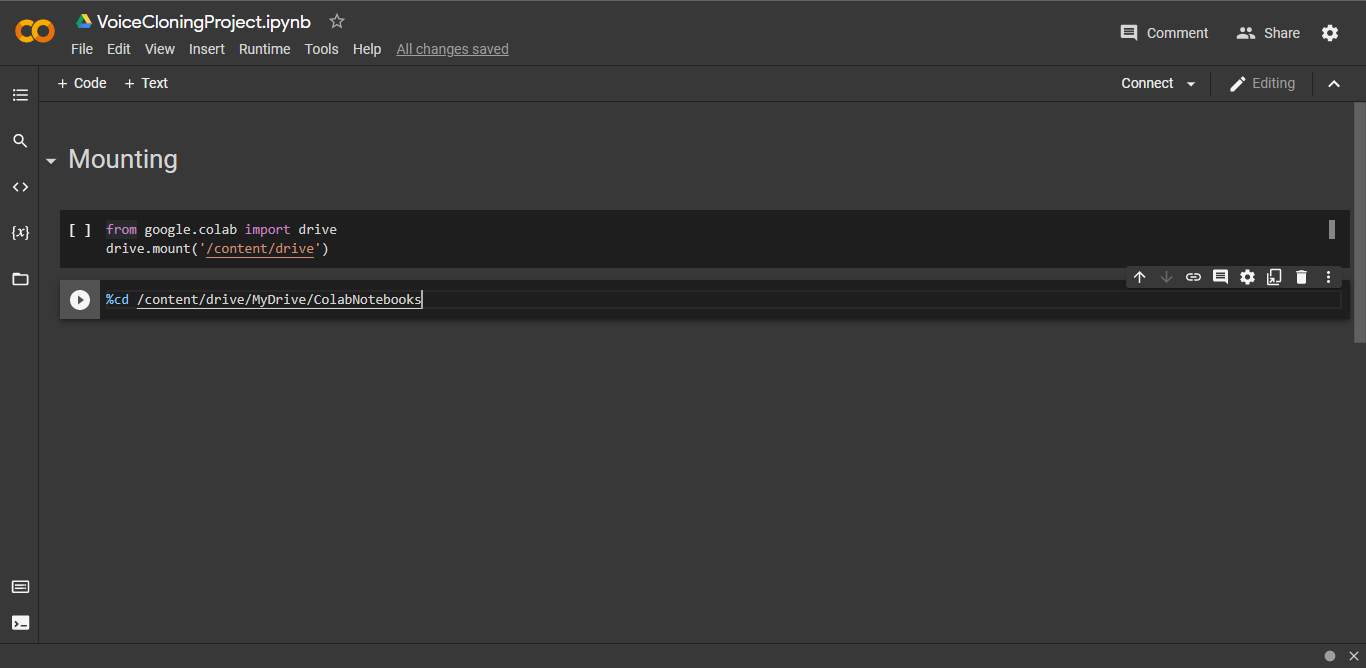
\includegraphics[scale=0.3]{figures/colab6}
=======
    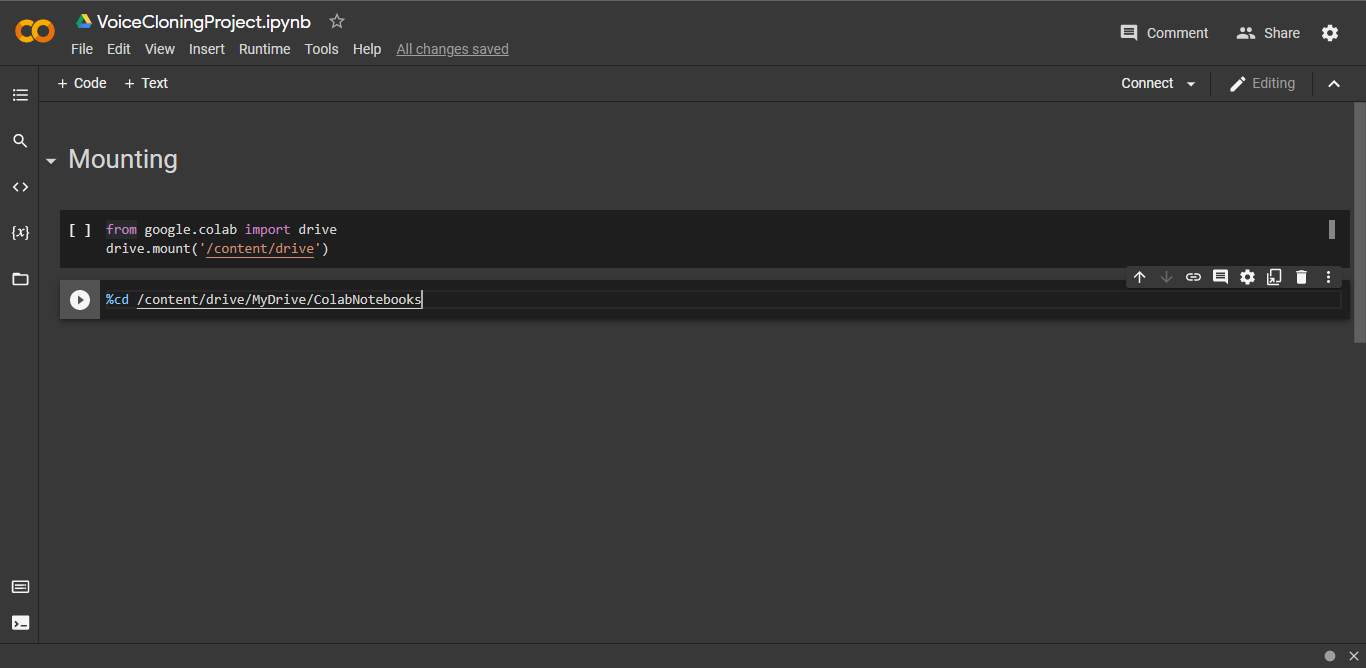
\includegraphics[scale=0.5]{figures/colab6}
>>>>>>> dd7a028f1952c03bff23c6357309752cba9024eb
    \caption{\textit{Change Directory}}
    \label{colab6}
\end{figure}

\item Tambahkan lagi text dan ketikkan \#Clone Repository lalu klik code untuk menambahkan kode berikut ini untuk clone repository dari github dan menginstall semua library yang ada di file requirements.txt.

\begin{lstlisting}[language=Python, caption=Clone Repository]
%tensorflow_version 1.x
import os
from os.path import exists, join, basename, splitext

git_repo_url = 'https://github.com/dindamajesty13/Real-Time-Voice-Cloning.git'
project_name = splitext(basename(git_repo_url))[0]
if not exists(project_name):
  # clone and install
  !git clone -q --recursive {git_repo_url}
  # install dependencies
  !cd {project_name} && pip install -q -r requirements.txt
  !pip install -q gdown
  !apt-get install -qq libportaudio2
  !pip install -q https://github.com/tugstugi/dl-colab-notebooks/archive/colab_utils.zip
\end{lstlisting}

Silahkan ganti git\_repo\_url dengan link repository teman-teman.

\begin{figure}[H]
    \centering
<<<<<<< HEAD
    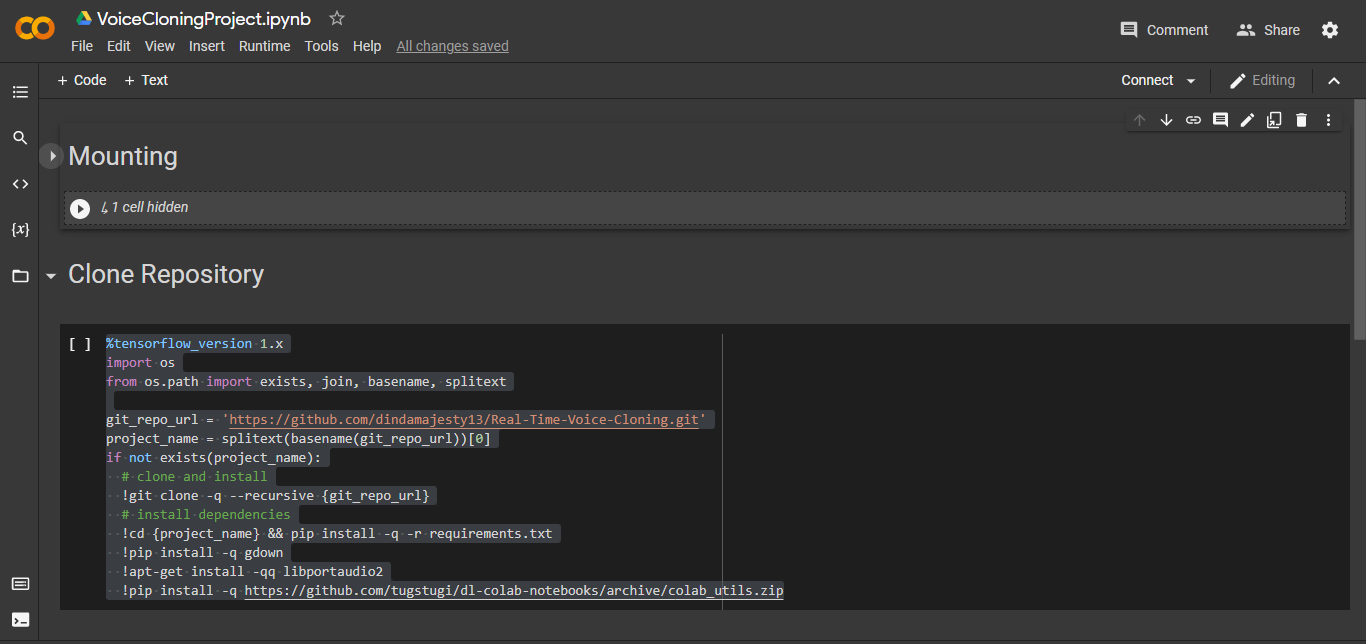
\includegraphics[scale=0.3]{figures/colab5}
=======
    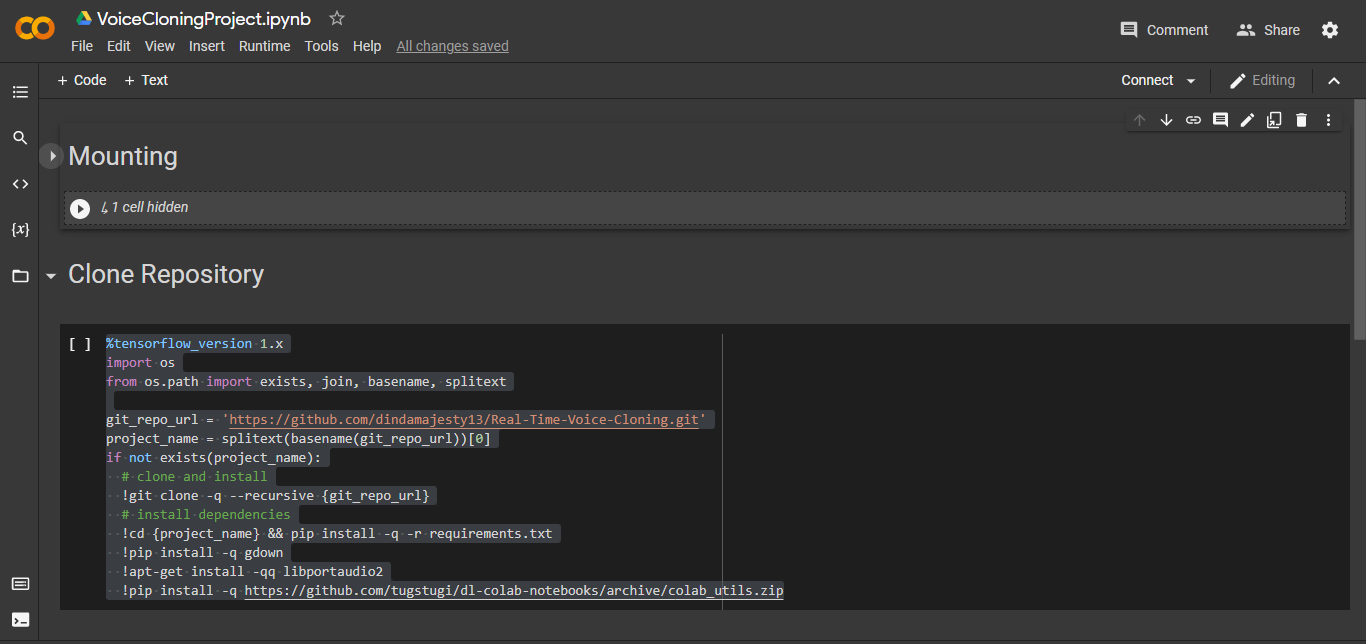
\includegraphics[scale=0.45]{figures/colab5}
>>>>>>> dd7a028f1952c03bff23c6357309752cba9024eb
    \caption{\textit{Script Clone Repository}}
    \label{colab5}
\end{figure}

\item Apabila Clone Project telah selesai maka klik icon folder di kiri tampilan google colab teman-teman lalu cari folder Real-Time-Voice-Cloning untuk memastikan bahwa repositori telah berhasil di clone.
\begin{figure}[H]
    \centering
<<<<<<< HEAD
    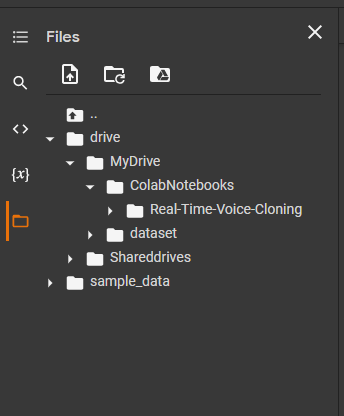
\includegraphics[scale=0.65]{figures/colab7}
=======
    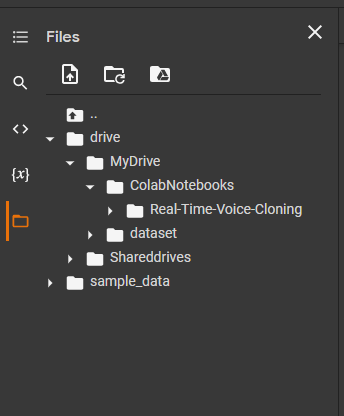
\includegraphics[scale=0.75]{figures/colab7}
>>>>>>> dd7a028f1952c03bff23c6357309752cba9024eb
    \caption{\textit{Check Folder}}
    \label{clab7}
\end{figure}

\item Buka file config.py yang terdapat didalam folder encoder, edit kode berikut sesuai dengan dataset yang teman-teman gunakan. Ganti value dari key clean sesuai dengan nama folder tempat teman-teman menyimpan dataset. Jika teman-teman hanya menggunakan satu dataset maka cukup abaikan salah satunya. Saya sarankan teman-teman mengganti nama variabel sesuai dengan dataset teman-teman.

\begin{lstlisting}[language=Python, caption=Config Dataset]
#dataset 1
common_voice = {
    "train": {
        "clean": ["common_voice"]
    },
    "test": {
        "clean": ["test_clean_data"]
    },
}

#dataset 2
titml_datasets = {
    "train": {
        "clean": ["titml"]
    },
    "test": {
        "clean": ["wwDataset"]
    },
}

#contoh
nama_dataset = {
    "train": {
        "clean": ["nama_folder_dataset"]
    },
    "test": {
        "clean": ["nama_folder_dataset"]
    },
}
\end{lstlisting}

\item Buka file preprocess.py yang ada didalam folder encoder lalu edit kode berikut, sesuaikan dengan dataset yang teman-teman gunakan.
\begin{lstlisting}[language=Python, caption=Preprocessing Function]
#import dataset sesuai dengan nama dataset pada config.py
#jika hanya satu dataset saja cukup importkan satu dataset, jika lebih dari dua maka importkan dan pisahkan dengan koma

from encoder.config import common_voice, titml_datasets

#ganti common_voice menjadi nama dataset pada config.py dan sesuaikan dengan yang diimportkan
#ganti wav sesuai dengan ekstensi file audio dataset teman-teman (mp3, flac, wav, m4a)

def preprocess_clean_dataset(datasets_root: Path, out_dir: Path, skip_existing=False):
    for dataset_name in common_voice["train"]["clean"]:
        # Initialize the preprocessing
        dataset_root, logger = _init_preprocess_dataset(dataset_name, datasets_root, out_dir)
        if not dataset_root:
            return

            # Preprocess all speakers
        speaker_dirs = list(dataset_root.glob("*"))
        _preprocess_speaker_dirs(speaker_dirs, dataset_name, datasets_root, out_dir, "wav",
                                 skip_existing, logger)

#sama dengan diatas.
#catatan: jika teman-teman hanya menggunakan satu dataset maka hapus function ini, abaikan, atau komen.
#jika menggunakan tiga dataset maka tambahkan function ini dan sesuaikan dengan dataset teman-teman seperti cara di atas.

def preprocess_speech_dataset(datasets_root: Path, out_dir: Path, skip_existing=False):
    for dataset_name in titml_datasets["train"]["clean"]:
        # Initialize the preprocessing
        dataset_root, logger = _init_preprocess_dataset(dataset_name, datasets_root, out_dir)
        if not dataset_root:
            return

            # Preprocess all speakers
        speaker_dirs = list(dataset_root.glob("*"))
        _preprocess_speaker_dirs(speaker_dirs, dataset_name, datasets_root, out_dir, "wav",
                                 skip_existing, logger)
\end{lstlisting}

\item Selanjutnya edit file encoder\_preprocessing.py seperti pada kode \ref{lstencoder}.

\begin{lstlisting}[language=Python, caption=Preprocessing Encoder Model, label=lstencoder]
from encoder.preprocess import preprocess_clean_dataset, preprocess_speech_dataset
from utils.argutils import print_args
from pathlib import Path
import argparse


if __name__ == "__main__":
    class MyFormatter(argparse.ArgumentDefaultsHelpFormatter, argparse.RawDescriptionHelpFormatter):
        pass

    parser = argparse.ArgumentParser(
        description="Preprocesses audio files from datasets, encodes them as mel spectrograms and "
                    "writes them to the disk. This will allow you to train the encoder. The "
                    "datasets required are at least one of VoxCeleb1, VoxCeleb2 and LibriSpeech. "
                    "Ideally, you should have all three. You should extract them as they are "
                    "after having downloaded them and put them in a same directory, e.g.:\n"
                    "-[datasets_root]\n"
                    "  -LibriSpeech\n"
                    "    -train-other-500\n"
                    "  -VoxCeleb1\n"
                    "    -wav\n"
                    "    -vox1_meta.csv\n"
                    "  -VoxCeleb2\n"
                    "    -dev",
        formatter_class=MyFormatter
    )
    parser.add_argument("datasets_root", type=Path, help=\
        "Path to the directory containing your LibriSpeech/TTS and VoxCeleb datasets.")
    parser.add_argument("-o", "--out_dir", type=Path, default=argparse.SUPPRESS, help=\
        "Path to the output directory that will contain the mel spectrograms. If left out, "
        "defaults to <datasets_root>/SV2TTS/encoder/")
    parser.add_argument("-d", "--datasets", type=str,
                        default="titml,common_voice", help=\
        "Comma-separated list of the name of the datasets you want to preprocess. Only the train "
        "set of these datasets will be used. Possible names: librispeech_other, voxceleb1, "
        "voxceleb2.")
    parser.add_argument("-s", "--skip_existing", action="store_true", help=\
        "Whether to skip existing output files with the same name. Useful if this script was "
        "interrupted.")
    parser.add_argument("--no_trim", action="store_true", help=\
        "Preprocess audio without trimming silences (not recommended).")
    args = parser.parse_args()

    # Verify webrtcvad is available
    if not args.no_trim:
        try:
            import webrtcvad
        except:
            raise ModuleNotFoundError("Package 'webrtcvad' not found. This package enables "
                "noise removal and is recommended. Please install and try again. If installation fails, "
                "use --no_trim to disable this error message.")
    del args.no_trim

    # Process the arguments
    args.datasets = args.datasets.split(",")
    if not hasattr(args, "out_dir"):
        args.out_dir = args.datasets_root.joinpath("SV2TTS", "encoder")
    assert args.datasets_root.exists()
    args.out_dir.mkdir(exist_ok=True, parents=True)

    # Preprocess the datasets
    print_args(args, parser)
    preprocess_func = {
      "titml": preprocess_speech_dataset,
      "common_voice": preprocess_clean_dataset, 
    }
    args = vars(args)
    for dataset in args.pop("datasets"):
        print("Preprocessing %s" % dataset)
        preprocess_func[dataset](**args)
\end{lstlisting}

Pada argument dataset masukkan nama dataset yang teman-teman gunakan, pada kode diatas saya menggunakan dataset titml dan common voice berbahasa indonesia.

\item Upload dataset teman-teman ke google drive dengan struktur direktori seperti gambar \ref{colab9}
\begin{figure}[H]
    \centering
    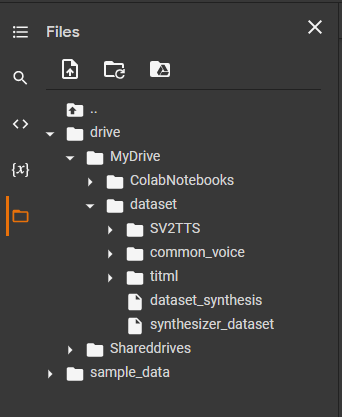
\includegraphics[scale=0.75]{figures/colab9}
    \caption{\textit{Struktur Dataset}}
    \label{colab9}
\end{figure}

\item Tambahkan text dan ketikkan \#Preprocessing encoder lalu tambahkan kode dan ketikkan kode program untuk menjalankan preprocessing speaker encoder model.

\begin{lstlisting}[language=Python, caption=Script to Run Preprocessing Speaker Encoder Model]
!python /content/drive/MyDrive/ColabNotebooks/Real-Time-Voice-Cloning/encoder_preprocess.py /content/drive/MyDrive/dataset
\end{lstlisting}

\begin{figure}[H]
    \centering
    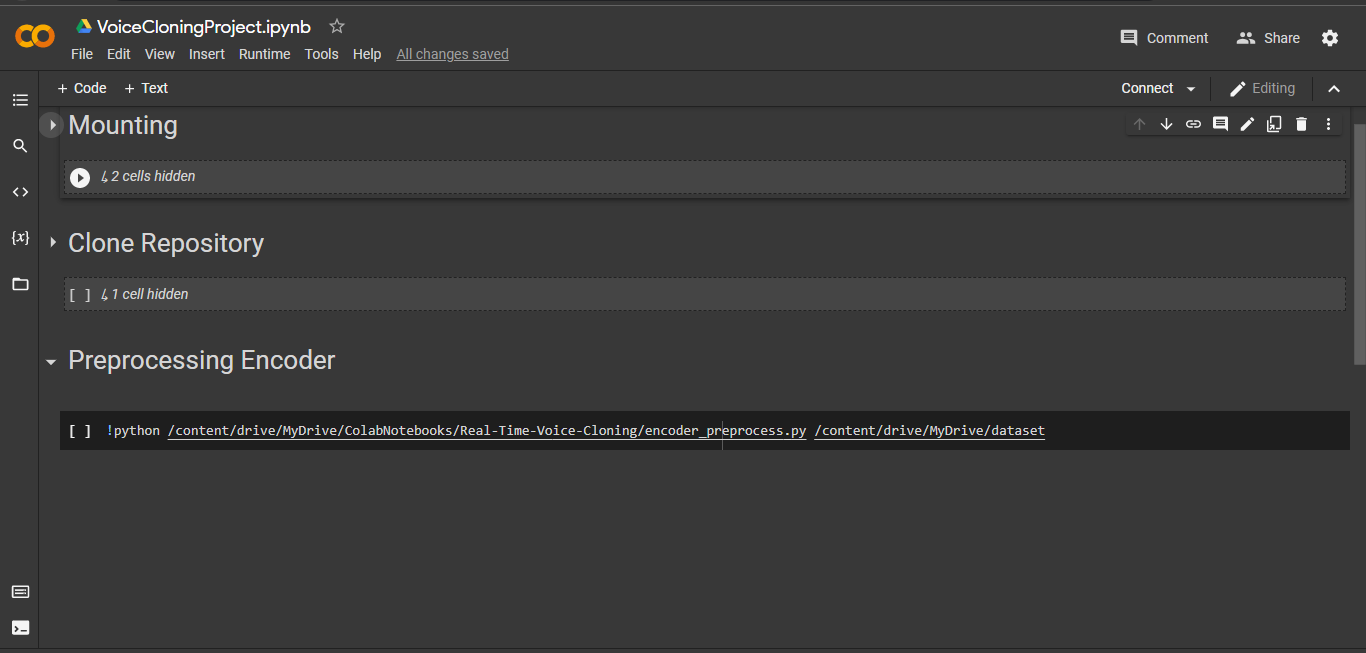
\includegraphics[scale=0.3]{figures/colab8}
    \caption{\textit{Preprocessing Speaker Encoder Model}}
    \label{colab8}
\end{figure}

\item Buka file encoder\_train.py lalu edit argument --model\_dir, pada bagian default isikan path direktori tempat model encoder akan disimpan.

\begin{lstlisting}[language=Python, caption=Training Speaker Encoder Model]
from utils.argutils import print_args
from encoder.train import train
from pathlib import Path
import argparse


if __name__ == "__main__":
    parser = argparse.ArgumentParser(
        description="Trains the speaker encoder. You must have run encoder_preprocess.py first.",
        formatter_class=argparse.ArgumentDefaultsHelpFormatter
    )
    
    parser.add_argument("run_id", type=str, help= \
        "Name for this model instance. If a model state from the same run ID was previously "
        "saved, the training will restart from there. Pass -f to overwrite saved states and "
        "restart from scratch.")
    parser.add_argument("clean_data_root", type=Path, help= \
        "Path to the output directory of encoder_preprocess.py. If you left the default "
        "output directory when preprocessing, it should be <datasets_root>/SV2TTS/encoder/.")
    parser.add_argument("-m", "--models_dir", type=Path, default="/content/drive/MyDrive/ColabNotebooks/Real-Time-Voice-Cloning/encoder/saved_models/", help=\
        "Path to the output directory that will contain the saved model weights, as well as "
        "backups of those weights and plots generated during training.")
    parser.add_argument("-v", "--vis_every", type=int, default=10, help= \
        "Number of steps between updates of the loss and the plots.")
    parser.add_argument("-u", "--umap_every", type=int, default=100, help= \
        "Number of steps between updates of the umap projection. Set to 0 to never update the "
        "projections.")
    parser.add_argument("-s", "--save_every", type=int, default=500, help= \
        "Number of steps between updates of the model on the disk. Set to 0 to never save the "
        "model.")
    parser.add_argument("-b", "--backup_every", type=int, default=7500, help= \
        "Number of steps between backups of the model. Set to 0 to never make backups of the "
        "model.")
    parser.add_argument("-f", "--force_restart", action="store_true", help= \
        "Do not load any saved model.")
    parser.add_argument("--visdom_server", type=str, default="http://localhost")
    parser.add_argument("--no_visdom", action="store_true", help= \
        "Disable visdom.")
    args = parser.parse_args()
    
    # Process the arguments
    args.models_dir.mkdir(exist_ok=True)
    
    # Run the training
    print_args(args, parser)
    train(**vars(args))
    
\end{lstlisting}

\item Selanjutnya, klik tambahkan text dan ketikkan \#Training encoder lalu klik tambahkan kode dan ketikkan kode program untuk menjalankan training speaker encoder model. Tambahkan argument --no\_visdom apabila teman-teman tidak menggunakan visdom server untuk menampilkan visualisasi dari hasil training speaker encoder model.

\begin{lstlisting}[language=Python, caption=Script to Run Training Speaker Encoder Model]
!python /content/drive/MyDrive/ColabNotebooks/Real-Time-Voice-Cloning/encoder_train.py pretrained /content/drive/MyDrive/dataset/SV2TTS/encoder/ --no_visdom
\end{lstlisting}

\begin{figure}[H]
    \centering
    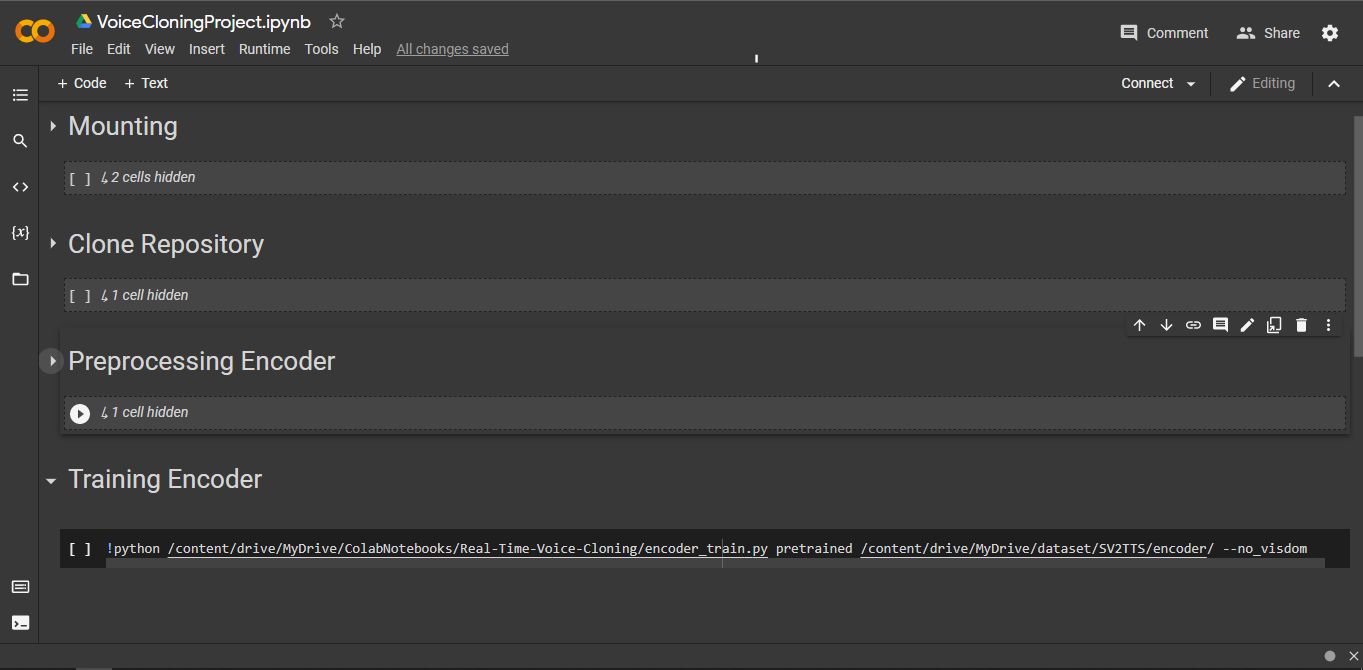
\includegraphics[scale=0.3]{figures/colab10}
    \caption{\textit{Training Speaker Encoder Model}}
    \label{colab10}
\end{figure}

\item Buka file synthesizer\_preprocess\_audio.py lalu edit argument --datasets\_name, pada bagian default isikan nama folder dataset teman-teman dan argumen --subfolders pada default isikan nama sub folder dari folder dataset. Jika terdapat lebih dari satu subfolder maka pisahkan subfolder 1 dan 2 menggunakan koma.

\begin{lstlisting}[language=Python, caption=Training Speaker Encoder Model]
from synthesizer.preprocess import preprocess_dataset
from synthesizer.hparams import hparams
from utils.argutils import print_args
from pathlib import Path
import argparse


if __name__ == "__main__":
    parser = argparse.ArgumentParser(
        description="Preprocesses audio files from datasets, encodes them as mel spectrograms "
                    "and writes them to  the disk. Audio files are also saved, to be used by the "
                    "vocoder for training.",
        formatter_class=argparse.ArgumentDefaultsHelpFormatter
    )
    parser.add_argument("datasets_root", type=Path, help=\
        "Path to the directory containing your LibriSpeech/TTS datasets.")
    parser.add_argument("-o", "--out_dir", type=Path, default=argparse.SUPPRESS, help=\
        "Path to the output directory that will contain the mel spectrograms, the audios and the "
        "embeds. Defaults to <datasets_root>/SV2TTS/synthesizer/")
    parser.add_argument("-n", "--n_processes", type=int, default=4, help=\
        "Number of processes in parallel.")
    parser.add_argument("-s", "--skip_existing", action="store_true", help=\
        "Whether to overwrite existing files with the same name. Useful if the preprocessing was "
        "interrupted.")
    parser.add_argument("--hparams", type=str, default="", help=\
        "Hyperparameter overrides as a comma-separated list of name-value pairs")
    parser.add_argument("--no_alignments", action="store_true", help=\
        "Use this option when dataset does not include alignments\
        (these are used to split long audio files into sub-utterances.)")
    parser.add_argument("--datasets_name", type=str, default="synthesizer_dataset", help=\
        "Name of the dataset directory to process.")
    parser.add_argument("--subfolders", type=str, default="cv-corpus-7.0-2021-07-21", help=\
        "Comma-separated list of subfolders to process inside your dataset directory")
    args = parser.parse_args()

    # Process the arguments
    if not hasattr(args, "out_dir"):
        args.out_dir = args.datasets_root.joinpath("SV2TTS", "synthesizer")

    # Create directories
    assert args.datasets_root.exists()
    args.out_dir.mkdir(exist_ok=True, parents=True)

    # Preprocess the dataset
    print_args(args, parser)
    args.hparams = hparams.parse(args.hparams)
    preprocess_dataset(**vars(args))
    
\end{lstlisting}

Berikut struktur folder dataset yang saya gunakan:
\begin{figure}[H]
    \centering
    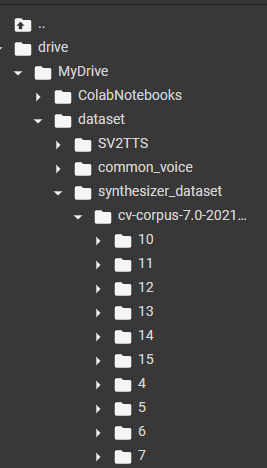
\includegraphics[scale=0.75]{figures/colab11}
    \caption{\textit{Struktur Folder Dataset Synthesizer}}
    \label{colab11}
\end{figure}

\item Selanjutnya, klik tambahkan text dan ketikkan \#Preprocessing Audio lalu klik tambahkan kode dan ketikkan kode program untuk menjalankan preprocessing audio. Tambahkan argumen --no\_alignments jika dataset yang teman-teman gunakan tidak memiliki alignments.

\begin{lstlisting}[language=Python, caption=Preprocessing Audio]
!python /content/drive/MyDrive/ColabNotebooks/Real-Time-Voice-Cloning/synthesizer_preprocess_audio.py /content/drive/MyDrive/dataset --no_alignments
\end{lstlisting}

\begin{figure}[H]
    \centering
    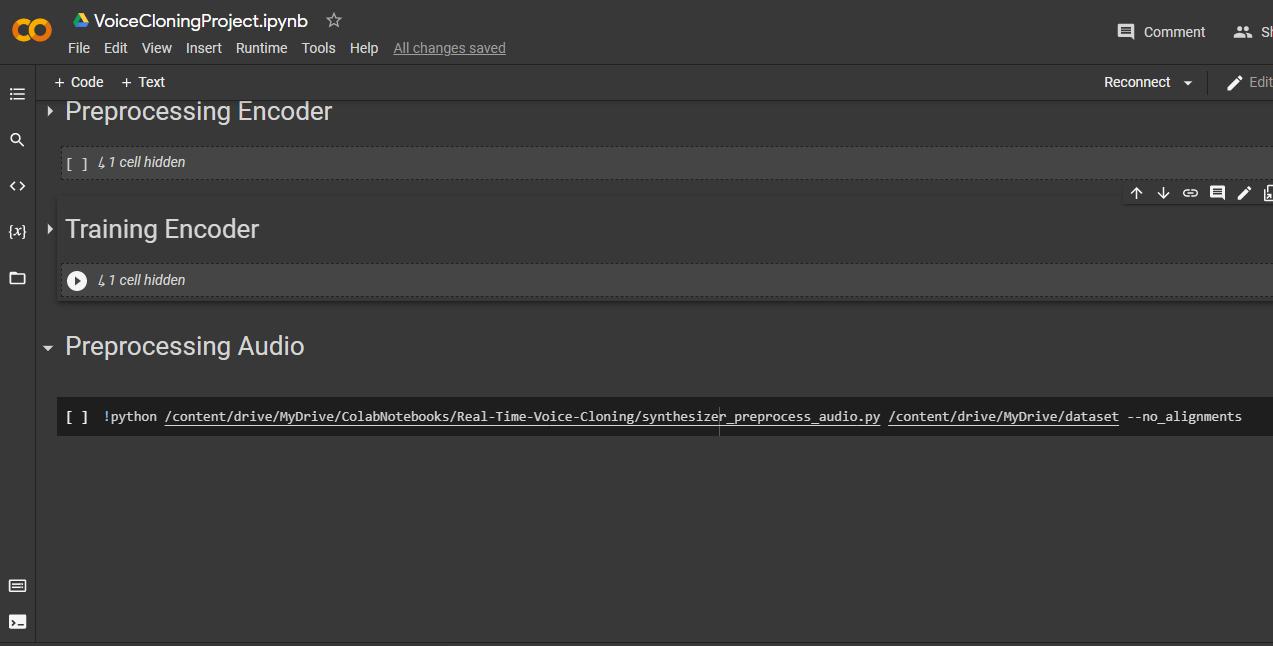
\includegraphics[scale=0.3]{figures/colab12}
    \caption{\textit{Preprocessing Audio}}
    \label{colab12}
\end{figure}

\item Buka file synthesizer\_preprocess\_embed.py lalu edit pada bagian argument --encoder\_model\_fpath dan isikan lokasi penyimpanan model speaker encoder yang telah di training sebelumnya pada bagian defaults.

\begin{lstlisting}[language=Python, caption=Training Speaker Encoder Model]
from synthesizer.preprocess import create_embeddings
from utils.argutils import print_args
from pathlib import Path
import argparse


if __name__ == "__main__":
    parser = argparse.ArgumentParser(
        description="Creates embeddings for the synthesizer from the LibriSpeech utterances.",
        formatter_class=argparse.ArgumentDefaultsHelpFormatter
    )
    parser.add_argument("synthesizer_root", type=Path, help=\
        "Path to the synthesizer training data that contains the audios and the train.txt file. "
        "If you let everything as default, it should be <datasets_root>/SV2TTS/synthesizer/.")
    parser.add_argument("-e", "--encoder_model_fpath", type=Path,
                        default="/content/drive/MyDrive/ColabNotebooks/Real-Time-Voice-Cloning/encoder/saved_models/pretrained.pt", help=\
        "Path your trained encoder model.")
    parser.add_argument("-n", "--n_processes", type=int, default=4, help= \
        "Number of parallel processes. An encoder is created for each, so you may need to lower "
        "this value on GPUs with low memory. Set it to 1 if CUDA is unhappy.")
    args = parser.parse_args()

    # Preprocess the dataset
    print_args(args, parser)
    create_embeddings(**vars(args))
    
\end{lstlisting}

\item Selanjutnya, klik tambahkan text dan ketikkan \#Preprocessing Embeds lalu klik tambahkan kode dan ketikkan kode program untuk menjalankan preprocessing audio embeddings. 

\begin{lstlisting}[language=Python, caption=Preprocessing Embeds]
!python /content/drive/MyDrive/ColabNotebooks/Real-Time-Voice-Cloning/synthesizer_preprocess_embeds.py /content/drive/MyDrive/dataset/SV2TTS/synthesizer
\end{lstlisting}

\begin{figure}[H]
    \centering
    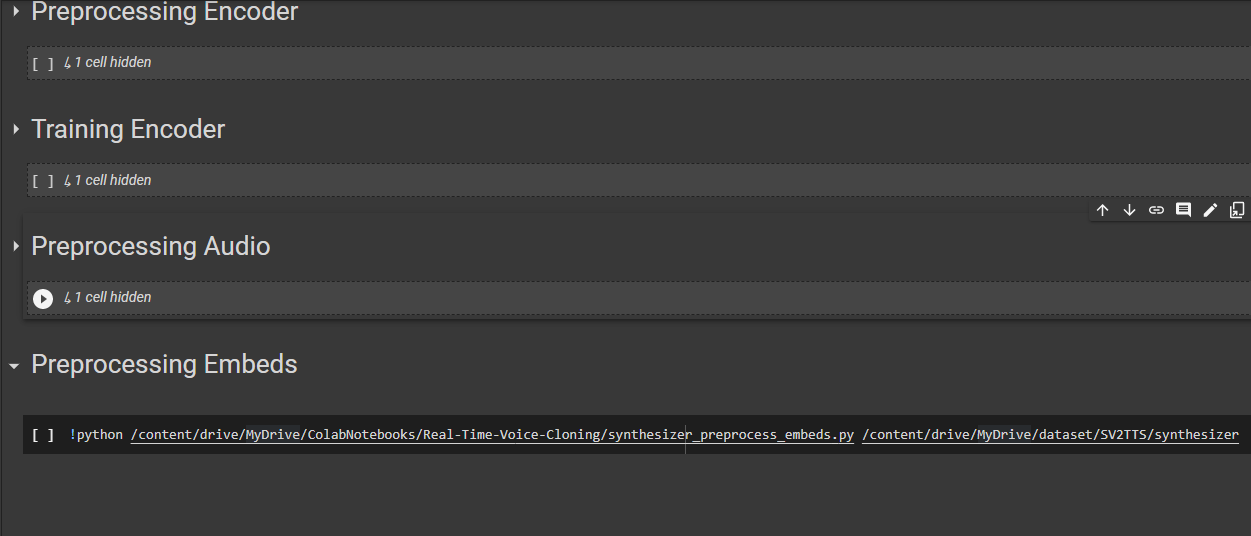
\includegraphics[scale=0.33]{figures/colab13}
    \caption{\textit{Preprocessing Audio Embeddings}}
    \label{colab13}
\end{figure}

\item Buka file synthesizer\_train.py lalu edit argument --models\_dir, pada bagian default isikan lokasi penyimpanan hasil training model synthesizer.

\begin{lstlisting}[language=Python, caption=Training Speaker Encoder Model]
from pathlib import Path

from synthesizer.hparams import hparams
from synthesizer.train import train
from utils.argutils import print_args
import argparse


if __name__ == "__main__":
    parser = argparse.ArgumentParser()
    parser.add_argument("run_id", type=str, help= \
        "Name for this model. By default, training outputs will be stored to saved_models/<run_id>/. If a model state "
        "from the same run ID was previously saved, the training will restart from there. Pass -f to overwrite saved "
        "states and restart from scratch.")
    parser.add_argument("syn_dir", type=Path, help= \
        "Path to the synthesizer directory that contains the ground truth mel spectrograms, "
        "the wavs and the embeds.")
    parser.add_argument("-m", "--models_dir", type=Path, default="/content/drive/MyDrive/ColabNotebooks/Real-Time-Voice-Cloning/synthesizer/saved_models", help=\
        "Path to the output directory that will contain the saved model weights and the logs.")
    parser.add_argument("-s", "--save_every", type=int, default=1000, help= \
        "Number of steps between updates of the model on the disk. Set to 0 to never save the "
        "model.")
    parser.add_argument("-b", "--backup_every", type=int, default=25000, help= \
        "Number of steps between backups of the model. Set to 0 to never make backups of the "
        "model.")
    parser.add_argument("-f", "--force_restart", action="store_true", help= \
        "Do not load any saved model and restart from scratch.")
    parser.add_argument("--hparams", default="", help=\
        "Hyperparameter overrides as a comma-separated list of name=value pairs")
    args = parser.parse_args()
    print_args(args, parser)

    args.hparams = hparams.parse(args.hparams)

    # Run the training
    train(**vars(args))
    
\end{lstlisting}

\item Selanjutnya, klik tambahkan text dan ketikkan \#Training Synthesizer Model lalu klik tambahkan kode dan ketikkan kode program untuk menjalankan proses training synthesizer model. 

\begin{lstlisting}[language=Python, caption=Training Synthesizer Model]
!python /content/drive/MyDrive/ColabNotebooks/Real-Time-Voice-Cloning/synthesizer_train.py pretrained /content/drive/MyDrive/dataset/SV2TTS/synthesizer
\end{lstlisting}

\begin{figure}[H]
    \centering
    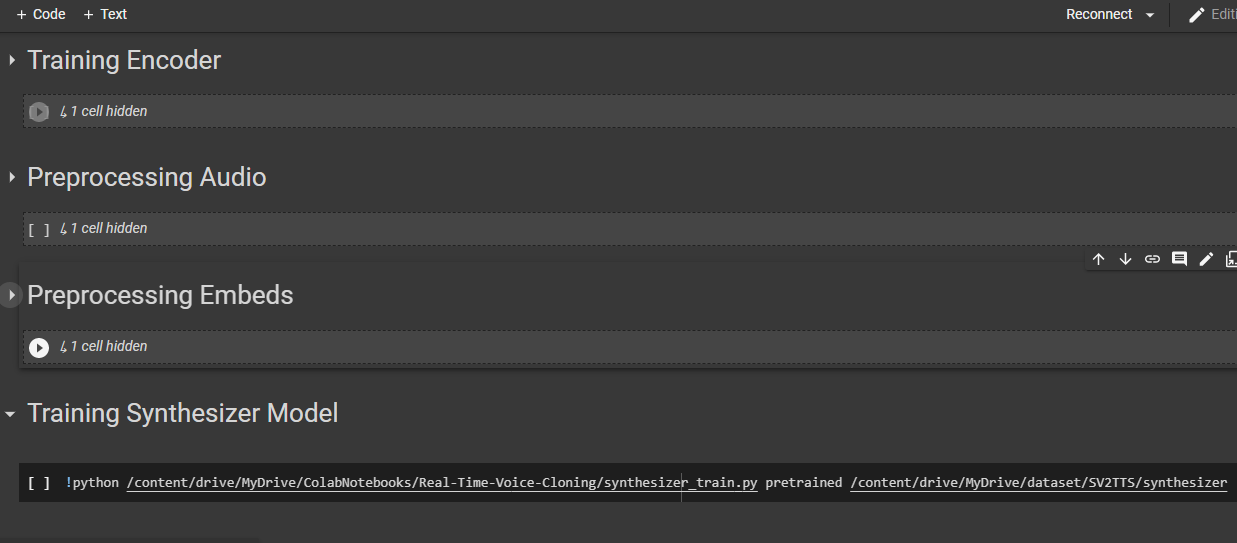
\includegraphics[scale=0.33]{figures/colab14}
    \caption{\textit{Training Synthesizer Model}}
    \label{colab14}
\end{figure}

\item Buka file vocoder\_preprocess.py lalu edit argument--syn\_model\_fpath, pada bagian default isikan lokasi penyimpanan hasil training model synthesizer.

\begin{lstlisting}[language=Python, caption=Vocoder Preprocess]
import argparse
import os
from pathlib import Path

from synthesizer.hparams import hparams
from synthesizer.synthesize import run_synthesis
from utils.argutils import print_args


if __name__ == "__main__":
    class MyFormatter(argparse.ArgumentDefaultsHelpFormatter, argparse.RawDescriptionHelpFormatter):
        pass

    parser = argparse.ArgumentParser(
        description="Creates ground-truth aligned (GTA) spectrograms from the vocoder.",
        formatter_class=MyFormatter
    )
    parser.add_argument("datasets_root", type=Path, help=\
        "Path to the directory containing your SV2TTS directory. If you specify both --in_dir and "
        "--out_dir, this argument won't be used.")
    parser.add_argument("-s", "--syn_model_fpath", type=Path,
                        default="/content/drive/MyDrive/ColabNotebooks/Real-Time-Voice-Cloning/synthesizer/saved_models/pretrained/synthesizer.pt",
                        help="Path to a saved synthesizer")
    parser.add_argument("-i", "--in_dir", type=Path, default=argparse.SUPPRESS, help= \
        "Path to the synthesizer directory that contains the mel spectrograms, the wavs and the "
        "embeds. Defaults to  <datasets_root>/SV2TTS/synthesizer/.")
    parser.add_argument("-o", "--out_dir", type=Path, default=argparse.SUPPRESS, help= \
        "Path to the output vocoder directory that will contain the ground truth aligned mel "
        "spectrograms. Defaults to <datasets_root>/SV2TTS/vocoder/.")
    parser.add_argument("--hparams", default="", help=\
        "Hyperparameter overrides as a comma-separated list of name=value pairs")
    parser.add_argument("--cpu", action="store_true", help=\
        "If True, processing is done on CPU, even when a GPU is available.")
    args = parser.parse_args()
    print_args(args, parser)
    modified_hp = hparams.parse(args.hparams)

    if not hasattr(args, "in_dir"):
        args.in_dir = args.datasets_root / "SV2TTS" / "synthesizer"
    if not hasattr(args, "out_dir"):
        args.out_dir = args.datasets_root / "SV2TTS" / "vocoder"

    if args.cpu:
        # Hide GPUs from Pytorch to force CPU processing
        os.environ["CUDA_VISIBLE_DEVICES"] = "-1"

    run_synthesis(args.in_dir, args.out_dir, args.syn_model_fpath, modified_hp)
\end{lstlisting}

\item Selanjutnya, klik tambahkan text dan ketikkan \#Preprocessing Vocoder lalu klik tambahkan kode dan ketikkan kode program untuk menjalankan proses preprocessing vocoder model. 

\begin{lstlisting}[language=Python, caption=Preprocessing Vococder Model]
!python /content/drive/MyDrive/ColabNotebooks/Real-Time-Voice-Cloning/vocoder_preprocess.py /content/drive/MyDrive/dataset
\end{lstlisting}

\begin{figure}[H]
    \centering
    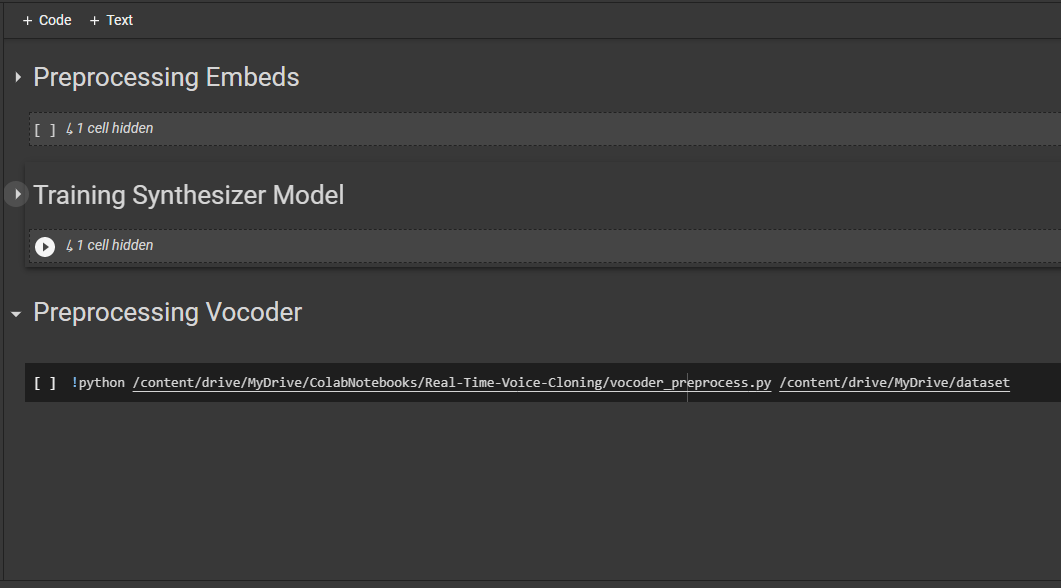
\includegraphics[scale=0.4]{figures/colab15}
    \caption{\textit{Preprocessing Vococder Model}}
    \label{colab14}
\end{figure}

\item Buka file vocoder\_train.py lalu edit argument --models\_dir, pada bagian default isikan lokasi untuk menyimpan hasil training vocoder model.

\begin{lstlisting}[language=Python, caption=Vocoder Train]
from utils.argutils import print_args
from vocoder.train import train
from pathlib import Path
import argparse


if __name__ == "__main__":
    parser = argparse.ArgumentParser(
        description="Trains the vocoder from the synthesizer audios and the GTA synthesized mels, "
                    "or ground truth mels.",
        formatter_class=argparse.ArgumentDefaultsHelpFormatter
    )
    
    parser.add_argument("run_id", type=str, help= \
        "Name for this model instance. If a model state from the same run ID was previously "
        "saved, the training will restart from there. Pass -f to overwrite saved states and "
        "restart from scratch.")
    parser.add_argument("datasets_root", type=str, help= \
        "Path to the directory containing your SV2TTS directory. Specifying --syn_dir or --voc_dir "
        "will take priority over this argument.")
    parser.add_argument("--syn_dir", type=str, default=argparse.SUPPRESS, help= \
        "Path to the synthesizer directory that contains the ground truth mel spectrograms, "
        "the wavs and the embeds. Defaults to <datasets_root>/SV2TTS/synthesizer/.")
    parser.add_argument("--voc_dir", type=str, default=argparse.SUPPRESS, help= \
        "Path to the vocoder directory that contains the GTA synthesized mel spectrograms. "
        "Defaults to <datasets_root>/SV2TTS/vocoder/. Unused if --ground_truth is passed.")
    parser.add_argument("-m", "--models_dir", type=str, default="/content/drive/MyDrive/ColabNotebooks/Real-Time-Voice-Cloning/vocoder/saved_models/", help=\
        "Path to the directory that will contain the saved model weights, as well as backups "
        "of those weights and wavs generated during training.")
    parser.add_argument("-g", "--ground_truth", action="store_true", help= \
        "Train on ground truth spectrograms (<datasets_root>/SV2TTS/synthesizer/mels).")
    parser.add_argument("-s", "--save_every", type=int, default=1000, help= \
        "Number of steps between updates of the model on the disk. Set to 0 to never save the "
        "model.")
    parser.add_argument("-b", "--backup_every", type=int, default=25000, help= \
        "Number of steps between backups of the model. Set to 0 to never make backups of the "
        "model.")
    parser.add_argument("-f", "--force_restart", action="store_true", help= \
        "Do not load any saved model and restart from scratch.")
    args = parser.parse_args()

    # Process the arguments
    if not hasattr(args, "syn_dir"):
        args.syn_dir = Path(args.datasets_root, "SV2TTS", "synthesizer")
    args.syn_dir = Path(args.syn_dir)
    if not hasattr(args, "voc_dir"):
        args.voc_dir = Path(args.datasets_root, "SV2TTS", "vocoder")
    args.voc_dir = Path(args.voc_dir)
    del args.datasets_root
    args.models_dir = Path(args.models_dir)
    args.models_dir.mkdir(exist_ok=True)

    # Run the training
    print_args(args, parser)
    train(**vars(args))
    
\end{lstlisting}

\item Selanjutnya, klik tambahkan text dan ketikkan \#Training Vocoder lalu klik tambahkan kode dan ketikkan kode program untuk menjalankan proses training vocoder model. Tambahkan argument --ground\_truth agar proses training dilakukan menggunakan mel spektrogram yang telah di preprocessing sebelumnya pada model synthesizer.

\begin{lstlisting}[language=Python, caption=Training Vococder Model]
!python /content/drive/MyDrive/ColabNotebooks/Real-Time-Voice-Cloning/vocoder_train.py pretrained /content/drive/MyDrive/dataset --ground_truth
\end{lstlisting}

\begin{figure}[H]
    \centering
    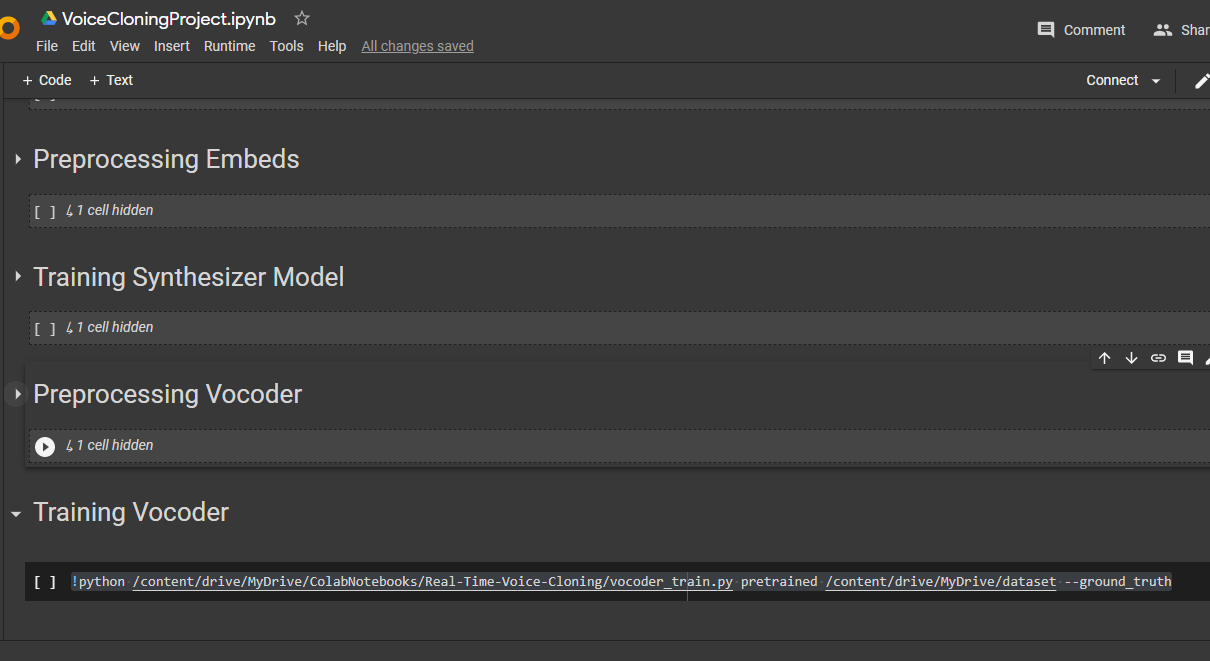
\includegraphics[scale=0.35]{figures/colab16}
    \caption{\textit{Training Vococder Model}}
    \label{colab15}
\end{figure}

\end{enumerate}